% Created by tikzDevice version 0.10.1 on 2016-06-29 14:28:51
% !TEX encoding = UTF-8 Unicode
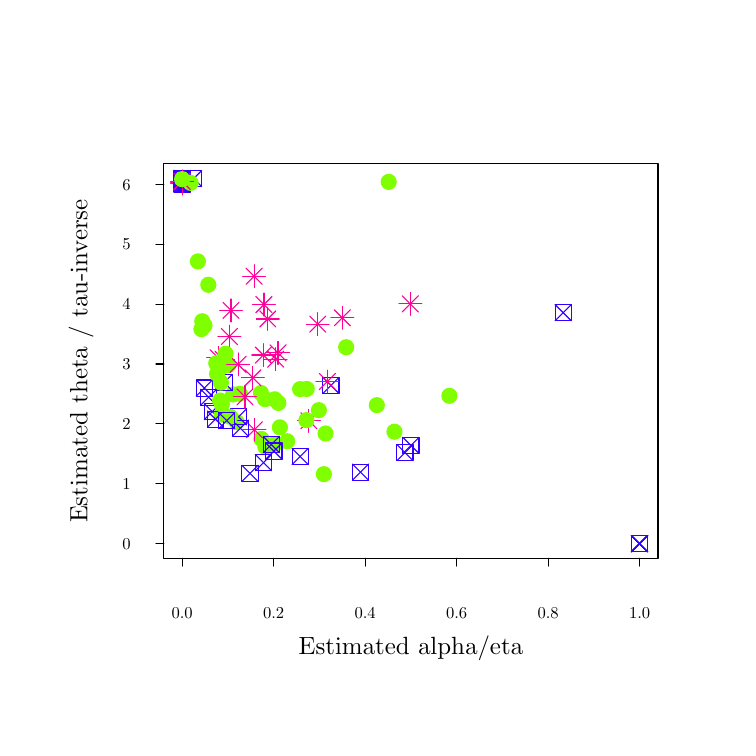
\begin{tikzpicture}[x=1pt,y=1pt]
\definecolor{fillColor}{RGB}{255,255,255}
\path[use as bounding box,fill=fillColor,fill opacity=0.00] (0,0) rectangle (252.94,252.94);
\begin{scope}
\path[clip] ( 49.20, 61.20) rectangle (227.75,203.75);
\definecolor{fillColor}{RGB}{128,255,0}

\path[fill=fillColor] ( 65.27,160.03) circle (  2.92);
\definecolor{drawColor}{RGB}{255,0,153}

\path[draw=drawColor,line width= 0.4pt,line join=round,line cap=round] ( 67.72,130.14) -- ( 73.57,135.99);

\path[draw=drawColor,line width= 0.4pt,line join=round,line cap=round] ( 67.72,135.99) -- ( 73.57,130.14);

\path[draw=drawColor,line width= 0.4pt,line join=round,line cap=round] ( 66.51,133.06) -- ( 74.79,133.06);

\path[draw=drawColor,line width= 0.4pt,line join=round,line cap=round] ( 70.65,128.92) -- ( 70.65,137.20);
\definecolor{drawColor}{RGB}{51,0,255}

\path[draw=drawColor,line width= 0.4pt,line join=round,line cap=round] (218.21, 63.55) rectangle (224.06, 69.40);

\path[draw=drawColor,line width= 0.4pt,line join=round,line cap=round] (218.21, 63.55) -- (224.06, 69.40);

\path[draw=drawColor,line width= 0.4pt,line join=round,line cap=round] (218.21, 69.40) -- (224.06, 63.55);

\path[draw=drawColor,line width= 0.4pt,line join=round,line cap=round] (106.64,120.75) rectangle (112.49,126.60);

\path[draw=drawColor,line width= 0.4pt,line join=round,line cap=round] (106.64,120.75) -- (112.49,126.60);

\path[draw=drawColor,line width= 0.4pt,line join=round,line cap=round] (106.64,126.60) -- (112.49,120.75);

\path[fill=fillColor] ( 84.30,120.93) circle (  2.92);

\path[draw=drawColor,line width= 0.4pt,line join=round,line cap=round] ( 60.90,119.78) rectangle ( 66.75,125.63);

\path[draw=drawColor,line width= 0.4pt,line join=round,line cap=round] ( 60.90,119.78) -- ( 66.75,125.63);

\path[draw=drawColor,line width= 0.4pt,line join=round,line cap=round] ( 60.90,125.63) -- ( 66.75,119.78);

\path[fill=fillColor] ( 89.36,102.54) circle (  2.92);

\path[fill=fillColor] (130.46,197.22) circle (  2.92);

\path[fill=fillColor] ( 90.59,117.35) circle (  2.92);
\definecolor{drawColor}{RGB}{255,0,153}

\path[draw=drawColor,line width= 0.4pt,line join=round,line cap=round] ( 65.90,130.71) -- ( 71.75,136.56);

\path[draw=drawColor,line width= 0.4pt,line join=round,line cap=round] ( 65.90,136.56) -- ( 71.75,130.71);

\path[draw=drawColor,line width= 0.4pt,line join=round,line cap=round] ( 64.69,133.63) -- ( 72.96,133.63);

\path[draw=drawColor,line width= 0.4pt,line join=round,line cap=round] ( 68.83,129.50) -- ( 68.83,137.77);

\path[fill=fillColor] ( 55.81,196.53) circle (  2.92);

\path[fill=fillColor] ( 84.47,104.33) circle (  2.92);

\path[fill=fillColor] ( 56.45,198.30) circle (  2.92);

\path[fill=fillColor] ( 74.23,120.40) circle (  2.92);
\definecolor{drawColor}{RGB}{51,0,255}

\path[draw=drawColor,line width= 0.4pt,line join=round,line cap=round] ( 52.89,193.54) rectangle ( 58.74,199.39);

\path[draw=drawColor,line width= 0.4pt,line join=round,line cap=round] ( 52.89,193.54) -- ( 58.74,199.39);

\path[draw=drawColor,line width= 0.4pt,line join=round,line cap=round] ( 52.89,199.39) -- ( 58.74,193.54);

\path[draw=drawColor,line width= 0.4pt,line join=round,line cap=round] ( 52.89,194.24) rectangle ( 58.74,200.09);

\path[draw=drawColor,line width= 0.4pt,line join=round,line cap=round] ( 52.89,194.24) -- ( 58.74,200.09);

\path[draw=drawColor,line width= 0.4pt,line join=round,line cap=round] ( 52.89,200.09) -- ( 58.74,194.24);
\definecolor{drawColor}{RGB}{255,0,153}

\path[draw=drawColor,line width= 0.4pt,line join=round,line cap=round] (101.89,142.86) -- (107.74,148.71);

\path[draw=drawColor,line width= 0.4pt,line join=round,line cap=round] (101.89,148.71) -- (107.74,142.86);

\path[draw=drawColor,line width= 0.4pt,line join=round,line cap=round] (100.68,145.78) -- (108.95,145.78);

\path[draw=drawColor,line width= 0.4pt,line join=round,line cap=round] (104.82,141.65) -- (104.82,149.92);
\definecolor{drawColor}{RGB}{51,0,255}

\path[draw=drawColor,line width= 0.4pt,line join=round,line cap=round] ( 62.47,116.45) rectangle ( 68.32,122.30);

\path[draw=drawColor,line width= 0.4pt,line join=round,line cap=round] ( 62.47,116.45) -- ( 68.32,122.30);

\path[draw=drawColor,line width= 0.4pt,line join=round,line cap=round] ( 62.47,122.30) -- ( 68.32,116.45);
\definecolor{drawColor}{RGB}{255,0,153}

\path[draw=drawColor,line width= 0.4pt,line join=round,line cap=round] ( 98.67,107.97) -- (104.52,113.82);

\path[draw=drawColor,line width= 0.4pt,line join=round,line cap=round] ( 98.67,113.82) -- (104.52,107.97);

\path[draw=drawColor,line width= 0.4pt,line join=round,line cap=round] ( 97.45,110.89) -- (105.73,110.89);

\path[draw=drawColor,line width= 0.4pt,line join=round,line cap=round] (101.59,106.75) -- (101.59,115.03);
\definecolor{drawColor}{RGB}{51,0,255}

\path[draw=drawColor,line width= 0.4pt,line join=round,line cap=round] ( 52.89,195.14) rectangle ( 58.74,200.99);

\path[draw=drawColor,line width= 0.4pt,line join=round,line cap=round] ( 52.89,195.14) -- ( 58.74,200.99);

\path[draw=drawColor,line width= 0.4pt,line join=round,line cap=round] ( 52.89,200.99) -- ( 58.74,195.14);

\path[draw=drawColor,line width= 0.4pt,line join=round,line cap=round] (218.09, 63.55) rectangle (223.94, 69.40);

\path[draw=drawColor,line width= 0.4pt,line join=round,line cap=round] (218.09, 63.55) -- (223.94, 69.40);

\path[draw=drawColor,line width= 0.4pt,line join=round,line cap=round] (218.09, 69.40) -- (223.94, 63.55);

\path[fill=fillColor] ( 76.68,120.65) circle (  2.92);

\path[fill=fillColor] ( 69.50,129.68) circle (  2.92);
\definecolor{drawColor}{RGB}{255,0,153}

\path[draw=drawColor,line width= 0.4pt,line join=round,line cap=round] ( 52.89,194.23) -- ( 58.74,200.08);

\path[draw=drawColor,line width= 0.4pt,line join=round,line cap=round] ( 52.89,200.08) -- ( 58.74,194.23);

\path[draw=drawColor,line width= 0.4pt,line join=round,line cap=round] ( 51.68,197.15) -- ( 59.95,197.15);

\path[draw=drawColor,line width= 0.4pt,line join=round,line cap=round] ( 55.81,193.02) -- ( 55.81,201.29);
\definecolor{drawColor}{RGB}{51,0,255}

\path[draw=drawColor,line width= 0.4pt,line join=round,line cap=round] ( 63.79,111.26) rectangle ( 69.64,117.11);

\path[draw=drawColor,line width= 0.4pt,line join=round,line cap=round] ( 63.79,111.26) -- ( 69.64,117.11);

\path[draw=drawColor,line width= 0.4pt,line join=round,line cap=round] ( 63.79,117.11) -- ( 69.64,111.26);
\definecolor{drawColor}{RGB}{255,0,153}

\path[draw=drawColor,line width= 0.4pt,line join=round,line cap=round] ( 52.89,193.64) -- ( 58.74,199.49);

\path[draw=drawColor,line width= 0.4pt,line join=round,line cap=round] ( 52.89,199.49) -- ( 58.74,193.64);

\path[draw=drawColor,line width= 0.4pt,line join=round,line cap=round] ( 51.68,196.57) -- ( 59.95,196.57);

\path[draw=drawColor,line width= 0.4pt,line join=round,line cap=round] ( 55.81,192.43) -- ( 55.81,200.70);

\path[fill=fillColor] ( 61.52,168.50) circle (  2.92);
\definecolor{drawColor}{RGB}{51,0,255}

\path[draw=drawColor,line width= 0.4pt,line join=round,line cap=round] (218.21, 63.55) rectangle (224.06, 69.40);

\path[draw=drawColor,line width= 0.4pt,line join=round,line cap=round] (218.21, 63.55) -- (224.06, 69.40);

\path[draw=drawColor,line width= 0.4pt,line join=round,line cap=round] (218.21, 69.40) -- (224.06, 63.55);

\path[fill=fillColor] ( 63.90,145.33) circle (  2.92);

\path[fill=fillColor] ( 89.26,118.65) circle (  2.92);
\definecolor{drawColor}{RGB}{255,0,153}

\path[draw=drawColor,line width= 0.4pt,line join=round,line cap=round] ( 78.46,123.48) -- ( 84.31,129.33);

\path[draw=drawColor,line width= 0.4pt,line join=round,line cap=round] ( 78.46,129.33) -- ( 84.31,123.48);

\path[draw=drawColor,line width= 0.4pt,line join=round,line cap=round] ( 77.24,126.41) -- ( 85.52,126.41);

\path[draw=drawColor,line width= 0.4pt,line join=round,line cap=round] ( 81.38,122.27) -- ( 81.38,130.55);

\path[fill=fillColor] ( 75.51,110.42) circle (  2.92);

\path[fill=fillColor] ( 85.88,101.50) circle (  2.92);

\path[draw=drawColor,line width= 0.4pt,line join=round,line cap=round] ( 69.96,138.39) -- ( 75.81,144.24);

\path[draw=drawColor,line width= 0.4pt,line join=round,line cap=round] ( 69.96,144.24) -- ( 75.81,138.39);

\path[draw=drawColor,line width= 0.4pt,line join=round,line cap=round] ( 68.75,141.31) -- ( 77.03,141.31);

\path[draw=drawColor,line width= 0.4pt,line join=round,line cap=round] ( 72.89,137.17) -- ( 72.89,145.45);

\path[fill=fillColor] (107.02, 91.60) circle (  2.92);
\definecolor{drawColor}{RGB}{51,0,255}

\path[draw=drawColor,line width= 0.4pt,line join=round,line cap=round] (218.21, 63.55) rectangle (224.06, 69.40);

\path[draw=drawColor,line width= 0.4pt,line join=round,line cap=round] (218.21, 63.55) -- (224.06, 69.40);

\path[draw=drawColor,line width= 0.4pt,line join=round,line cap=round] (218.21, 69.40) -- (224.06, 63.55);

\path[fill=fillColor] (105.22,114.72) circle (  2.92);

\path[draw=drawColor,line width= 0.4pt,line join=round,line cap=round] ( 52.89,193.74) rectangle ( 58.74,199.59);

\path[draw=drawColor,line width= 0.4pt,line join=round,line cap=round] ( 52.89,193.74) -- ( 58.74,199.59);

\path[draw=drawColor,line width= 0.4pt,line join=round,line cap=round] ( 52.89,199.59) -- ( 58.74,193.74);

\path[draw=drawColor,line width= 0.4pt,line join=round,line cap=round] (117.35, 89.40) rectangle (123.20, 95.25);

\path[draw=drawColor,line width= 0.4pt,line join=round,line cap=round] (117.35, 89.40) -- (123.20, 95.25);

\path[draw=drawColor,line width= 0.4pt,line join=round,line cap=round] (117.35, 95.25) -- (123.20, 89.40);

\path[draw=drawColor,line width= 0.4pt,line join=round,line cap=round] (133.40, 96.47) rectangle (139.25,102.32);

\path[draw=drawColor,line width= 0.4pt,line join=round,line cap=round] (133.40, 96.47) -- (139.25,102.32);

\path[draw=drawColor,line width= 0.4pt,line join=round,line cap=round] (133.40,102.32) -- (139.25, 96.47);

\path[draw=drawColor,line width= 0.4pt,line join=round,line cap=round] ( 68.06,121.77) rectangle ( 73.91,127.62);

\path[draw=drawColor,line width= 0.4pt,line join=round,line cap=round] ( 68.06,121.77) -- ( 73.91,127.62);

\path[draw=drawColor,line width= 0.4pt,line join=round,line cap=round] ( 68.06,127.62) -- ( 73.91,121.77);

\path[fill=fillColor] ( 72.52,130.97) circle (  2.92);

\path[draw=drawColor,line width= 0.4pt,line join=round,line cap=round] ( 52.89,194.98) rectangle ( 58.74,200.83);

\path[draw=drawColor,line width= 0.4pt,line join=round,line cap=round] ( 52.89,194.98) -- ( 58.74,200.83);

\path[draw=drawColor,line width= 0.4pt,line join=round,line cap=round] ( 52.89,200.83) -- ( 58.74,194.98);

\path[draw=drawColor,line width= 0.4pt,line join=round,line cap=round] ( 52.89,194.00) rectangle ( 58.74,199.85);

\path[draw=drawColor,line width= 0.4pt,line join=round,line cap=round] ( 52.89,194.00) -- ( 58.74,199.85);

\path[draw=drawColor,line width= 0.4pt,line join=round,line cap=round] ( 52.89,199.85) -- ( 58.74,194.00);
\definecolor{drawColor}{RGB}{255,0,153}

\path[draw=drawColor,line width= 0.4pt,line join=round,line cap=round] ( 73.09,128.38) -- ( 78.94,134.23);

\path[draw=drawColor,line width= 0.4pt,line join=round,line cap=round] ( 73.09,134.23) -- ( 78.94,128.38);

\path[draw=drawColor,line width= 0.4pt,line join=round,line cap=round] ( 71.88,131.31) -- ( 80.16,131.31);

\path[draw=drawColor,line width= 0.4pt,line join=round,line cap=round] ( 76.02,127.17) -- ( 76.02,135.44);

\path[fill=fillColor] ( 93.76,103.50) circle (  2.92);

\path[draw=drawColor,line width= 0.4pt,line join=round,line cap=round] ( 86.70,130.26) -- ( 92.55,136.11);

\path[draw=drawColor,line width= 0.4pt,line join=round,line cap=round] ( 86.70,136.11) -- ( 92.55,130.26);

\path[draw=drawColor,line width= 0.4pt,line join=round,line cap=round] ( 85.48,133.18) -- ( 93.76,133.18);

\path[draw=drawColor,line width= 0.4pt,line join=round,line cap=round] ( 89.62,129.05) -- ( 89.62,137.32);

\path[draw=drawColor,line width= 0.4pt,line join=round,line cap=round] (135.34,150.20) -- (141.19,156.05);

\path[draw=drawColor,line width= 0.4pt,line join=round,line cap=round] (135.34,156.05) -- (141.19,150.20);

\path[draw=drawColor,line width= 0.4pt,line join=round,line cap=round] (134.13,153.13) -- (142.41,153.13);

\path[draw=drawColor,line width= 0.4pt,line join=round,line cap=round] (138.27,148.99) -- (138.27,157.26);

\path[fill=fillColor] (126.16,116.54) circle (  2.92);
\definecolor{drawColor}{RGB}{51,0,255}

\path[draw=drawColor,line width= 0.4pt,line join=round,line cap=round] ( 52.89,195.54) rectangle ( 58.74,201.39);

\path[draw=drawColor,line width= 0.4pt,line join=round,line cap=round] ( 52.89,195.54) -- ( 58.74,201.39);

\path[draw=drawColor,line width= 0.4pt,line join=round,line cap=round] ( 52.89,201.39) -- ( 58.74,195.54);
\definecolor{drawColor}{RGB}{255,0,153}

\path[draw=drawColor,line width= 0.4pt,line join=round,line cap=round] ( 78.90,160.20) -- ( 84.75,166.05);

\path[draw=drawColor,line width= 0.4pt,line join=round,line cap=round] ( 78.90,166.05) -- ( 84.75,160.20);

\path[draw=drawColor,line width= 0.4pt,line join=round,line cap=round] ( 77.69,163.13) -- ( 85.96,163.13);

\path[draw=drawColor,line width= 0.4pt,line join=round,line cap=round] ( 81.83,158.99) -- ( 81.83,167.27);

\path[fill=fillColor] ( 70.07,113.13) circle (  2.92);

\path[fill=fillColor] ( 55.81,198.20) circle (  2.92);

\path[draw=drawColor,line width= 0.4pt,line join=round,line cap=round] (105.35,122.15) -- (111.20,128.00);

\path[draw=drawColor,line width= 0.4pt,line join=round,line cap=round] (105.35,128.00) -- (111.20,122.15);

\path[draw=drawColor,line width= 0.4pt,line join=round,line cap=round] (104.14,125.07) -- (112.41,125.07);

\path[draw=drawColor,line width= 0.4pt,line join=round,line cap=round] (108.27,120.94) -- (108.27,129.21);
\definecolor{drawColor}{RGB}{51,0,255}

\path[draw=drawColor,line width= 0.4pt,line join=round,line cap=round] (190.58,147.03) rectangle (196.43,152.88);

\path[draw=drawColor,line width= 0.4pt,line join=round,line cap=round] (190.58,147.03) -- (196.43,152.88);

\path[draw=drawColor,line width= 0.4pt,line join=round,line cap=round] (190.58,152.88) -- (196.43,147.03);

\path[draw=drawColor,line width= 0.4pt,line join=round,line cap=round] ( 52.89,194.31) rectangle ( 58.74,200.16);

\path[draw=drawColor,line width= 0.4pt,line join=round,line cap=round] ( 52.89,194.31) -- ( 58.74,200.16);

\path[draw=drawColor,line width= 0.4pt,line join=round,line cap=round] ( 52.89,200.16) -- ( 58.74,194.31);

\path[draw=drawColor,line width= 0.4pt,line join=round,line cap=round] ( 82.27, 92.85) rectangle ( 88.12, 98.70);

\path[draw=drawColor,line width= 0.4pt,line join=round,line cap=round] ( 82.27, 92.85) -- ( 88.12, 98.70);

\path[draw=drawColor,line width= 0.4pt,line join=round,line cap=round] ( 82.27, 98.70) -- ( 88.12, 92.85);

\path[fill=fillColor] ( 62.77,144.01) circle (  2.92);

\path[draw=drawColor,line width= 0.4pt,line join=round,line cap=round] ( 57.06,195.49) rectangle ( 62.91,201.34);

\path[draw=drawColor,line width= 0.4pt,line join=round,line cap=round] ( 57.06,195.49) -- ( 62.91,201.34);

\path[draw=drawColor,line width= 0.4pt,line join=round,line cap=round] ( 57.06,201.34) -- ( 62.91,195.49);

\path[draw=drawColor,line width= 0.4pt,line join=round,line cap=round] (218.21, 63.55) rectangle (224.06, 69.40);

\path[draw=drawColor,line width= 0.4pt,line join=round,line cap=round] (218.21, 63.55) -- (224.06, 69.40);

\path[draw=drawColor,line width= 0.4pt,line join=round,line cap=round] (218.21, 69.40) -- (224.06, 63.55);
\definecolor{drawColor}{RGB}{255,0,153}

\path[draw=drawColor,line width= 0.4pt,line join=round,line cap=round] ( 87.54,132.49) -- ( 93.39,138.34);

\path[draw=drawColor,line width= 0.4pt,line join=round,line cap=round] ( 87.54,138.34) -- ( 93.39,132.49);

\path[draw=drawColor,line width= 0.4pt,line join=round,line cap=round] ( 86.33,135.41) -- ( 94.60,135.41);

\path[draw=drawColor,line width= 0.4pt,line join=round,line cap=round] ( 90.47,131.27) -- ( 90.47,139.55);
\definecolor{drawColor}{RGB}{51,0,255}

\path[draw=drawColor,line width= 0.4pt,line join=round,line cap=round] ( 86.04, 97.00) rectangle ( 91.89,102.85);

\path[draw=drawColor,line width= 0.4pt,line join=round,line cap=round] ( 86.04, 97.00) -- ( 91.89,102.85);

\path[draw=drawColor,line width= 0.4pt,line join=round,line cap=round] ( 86.04,102.85) -- ( 91.89, 97.00);

\path[draw=drawColor,line width= 0.4pt,line join=round,line cap=round] ( 77.42, 88.97) rectangle ( 83.27, 94.82);

\path[draw=drawColor,line width= 0.4pt,line join=round,line cap=round] ( 77.42, 88.97) -- ( 83.27, 94.82);

\path[draw=drawColor,line width= 0.4pt,line join=round,line cap=round] ( 77.42, 94.82) -- ( 83.27, 88.97);

\path[draw=drawColor,line width= 0.4pt,line join=round,line cap=round] (218.09, 63.55) rectangle (223.94, 69.40);

\path[draw=drawColor,line width= 0.4pt,line join=round,line cap=round] (218.09, 63.55) -- (223.94, 69.40);

\path[draw=drawColor,line width= 0.4pt,line join=round,line cap=round] (218.09, 69.40) -- (223.94, 63.55);

\path[draw=drawColor,line width= 0.4pt,line join=round,line cap=round] ( 73.26,109.39) rectangle ( 79.11,115.24);

\path[draw=drawColor,line width= 0.4pt,line join=round,line cap=round] ( 73.26,109.39) -- ( 79.11,115.24);

\path[draw=drawColor,line width= 0.4pt,line join=round,line cap=round] ( 73.26,115.24) -- ( 79.11,109.39);

\path[fill=fillColor] ( 91.14,108.52) circle (  2.92);

\path[fill=fillColor] ( 85.77,118.71) circle (  2.92);
\definecolor{drawColor}{RGB}{255,0,153}

\path[draw=drawColor,line width= 0.4pt,line join=round,line cap=round] ( 52.89,194.32) -- ( 58.74,200.17);

\path[draw=drawColor,line width= 0.4pt,line join=round,line cap=round] ( 52.89,200.17) -- ( 58.74,194.32);

\path[draw=drawColor,line width= 0.4pt,line join=round,line cap=round] ( 51.68,197.25) -- ( 59.95,197.25);

\path[draw=drawColor,line width= 0.4pt,line join=round,line cap=round] ( 55.81,193.11) -- ( 55.81,201.38);

\path[fill=fillColor] (100.83,122.39) circle (  2.92);

\path[draw=drawColor,line width= 0.4pt,line join=round,line cap=round] ( 78.97,104.72) -- ( 84.82,110.57);

\path[draw=drawColor,line width= 0.4pt,line join=round,line cap=round] ( 78.97,110.57) -- ( 84.82,104.72);

\path[draw=drawColor,line width= 0.4pt,line join=round,line cap=round] ( 77.75,107.65) -- ( 86.03,107.65);

\path[draw=drawColor,line width= 0.4pt,line join=round,line cap=round] ( 81.89,103.51) -- ( 81.89,111.78);
\definecolor{drawColor}{RGB}{51,0,255}

\path[draw=drawColor,line width= 0.4pt,line join=round,line cap=round] ( 73.91,105.27) rectangle ( 79.76,111.12);

\path[draw=drawColor,line width= 0.4pt,line join=round,line cap=round] ( 73.91,105.27) -- ( 79.76,111.12);

\path[draw=drawColor,line width= 0.4pt,line join=round,line cap=round] ( 73.91,111.12) -- ( 79.76,105.27);
\definecolor{drawColor}{RGB}{255,0,153}

\path[draw=drawColor,line width= 0.4pt,line join=round,line cap=round] ( 83.83,144.75) -- ( 89.68,150.60);

\path[draw=drawColor,line width= 0.4pt,line join=round,line cap=round] ( 83.83,150.60) -- ( 89.68,144.75);

\path[draw=drawColor,line width= 0.4pt,line join=round,line cap=round] ( 82.62,147.68) -- ( 90.89,147.68);

\path[draw=drawColor,line width= 0.4pt,line join=round,line cap=round] ( 86.75,143.54) -- ( 86.75,151.81);

\path[fill=fillColor] ( 98.44,122.34) circle (  2.92);

\path[draw=drawColor,line width= 0.4pt,line join=round,line cap=round] ( 75.60,116.61) -- ( 81.45,122.46);

\path[draw=drawColor,line width= 0.4pt,line join=round,line cap=round] ( 75.60,122.46) -- ( 81.45,116.61);

\path[draw=drawColor,line width= 0.4pt,line join=round,line cap=round] ( 74.39,119.54) -- ( 82.66,119.54);

\path[draw=drawColor,line width= 0.4pt,line join=round,line cap=round] ( 78.53,115.40) -- ( 78.53,123.67);

\path[fill=fillColor] (115.09,137.47) circle (  2.92);
\definecolor{drawColor}{RGB}{51,0,255}

\path[draw=drawColor,line width= 0.4pt,line join=round,line cap=round] ( 52.89,195.45) rectangle ( 58.74,201.30);

\path[draw=drawColor,line width= 0.4pt,line join=round,line cap=round] ( 52.89,195.45) -- ( 58.74,201.30);

\path[draw=drawColor,line width= 0.4pt,line join=round,line cap=round] ( 52.89,201.30) -- ( 58.74,195.45);

\path[draw=drawColor,line width= 0.4pt,line join=round,line cap=round] (135.56, 99.07) rectangle (141.41,104.92);

\path[draw=drawColor,line width= 0.4pt,line join=round,line cap=round] (135.56, 99.07) -- (141.41,104.92);

\path[draw=drawColor,line width= 0.4pt,line join=round,line cap=round] (135.56,104.92) -- (141.41, 99.07);

\path[draw=drawColor,line width= 0.4pt,line join=round,line cap=round] ( 64.94,108.53) rectangle ( 70.79,114.38);

\path[draw=drawColor,line width= 0.4pt,line join=round,line cap=round] ( 64.94,108.53) -- ( 70.79,114.38);

\path[draw=drawColor,line width= 0.4pt,line join=round,line cap=round] ( 64.94,114.38) -- ( 70.79,108.53);
\definecolor{drawColor}{RGB}{255,0,153}

\path[draw=drawColor,line width= 0.4pt,line join=round,line cap=round] ( 70.55,147.83) -- ( 76.40,153.68);

\path[draw=drawColor,line width= 0.4pt,line join=round,line cap=round] ( 70.55,153.68) -- ( 76.40,147.83);

\path[draw=drawColor,line width= 0.4pt,line join=round,line cap=round] ( 69.34,150.76) -- ( 77.61,150.76);

\path[draw=drawColor,line width= 0.4pt,line join=round,line cap=round] ( 73.48,146.62) -- ( 73.48,154.89);
\definecolor{drawColor}{RGB}{51,0,255}

\path[draw=drawColor,line width= 0.4pt,line join=round,line cap=round] ( 52.89,195.13) rectangle ( 58.74,200.98);

\path[draw=drawColor,line width= 0.4pt,line join=round,line cap=round] ( 52.89,195.13) -- ( 58.74,200.98);

\path[draw=drawColor,line width= 0.4pt,line join=round,line cap=round] ( 52.89,200.98) -- ( 58.74,195.13);

\path[fill=fillColor] ( 73.17,112.34) circle (  2.92);

\path[fill=fillColor] ( 68.14,131.67) circle (  2.92);
\definecolor{drawColor}{RGB}{255,0,153}

\path[draw=drawColor,line width= 0.4pt,line join=round,line cap=round] ( 82.22,131.72) -- ( 88.07,137.57);

\path[draw=drawColor,line width= 0.4pt,line join=round,line cap=round] ( 82.22,137.57) -- ( 88.07,131.72);

\path[draw=drawColor,line width= 0.4pt,line join=round,line cap=round] ( 81.01,134.64) -- ( 89.29,134.64);

\path[draw=drawColor,line width= 0.4pt,line join=round,line cap=round] ( 85.15,130.51) -- ( 85.15,138.78);

\path[fill=fillColor] ( 58.88,196.86) circle (  2.92);

\path[draw=drawColor,line width= 0.4pt,line join=round,line cap=round] ( 52.89,194.47) -- ( 58.74,200.32);

\path[draw=drawColor,line width= 0.4pt,line join=round,line cap=round] ( 52.89,200.32) -- ( 58.74,194.47);

\path[draw=drawColor,line width= 0.4pt,line join=round,line cap=round] ( 51.68,197.39) -- ( 59.95,197.39);

\path[draw=drawColor,line width= 0.4pt,line join=round,line cap=round] ( 55.81,193.26) -- ( 55.81,201.53);

\path[fill=fillColor] ( 55.81,198.19) circle (  2.92);

\path[fill=fillColor] ( 70.18,116.84) circle (  2.92);
\definecolor{drawColor}{RGB}{51,0,255}

\path[draw=drawColor,line width= 0.4pt,line join=round,line cap=round] ( 85.13, 99.36) rectangle ( 90.98,105.21);

\path[draw=drawColor,line width= 0.4pt,line join=round,line cap=round] ( 85.13, 99.36) -- ( 90.98,105.21);

\path[draw=drawColor,line width= 0.4pt,line join=round,line cap=round] ( 85.13,105.21) -- ( 90.98, 99.36);

\path[fill=fillColor] (132.53,106.94) circle (  2.92);

\path[fill=fillColor] (107.64,106.30) circle (  2.92);

\path[fill=fillColor] ( 71.51,135.13) circle (  2.92);
\definecolor{drawColor}{RGB}{255,0,153}

\path[draw=drawColor,line width= 0.4pt,line join=round,line cap=round] ( 82.46,149.97) -- ( 88.31,155.82);

\path[draw=drawColor,line width= 0.4pt,line join=round,line cap=round] ( 82.46,155.82) -- ( 88.31,149.97);

\path[draw=drawColor,line width= 0.4pt,line join=round,line cap=round] ( 81.25,152.90) -- ( 89.52,152.90);

\path[draw=drawColor,line width= 0.4pt,line join=round,line cap=round] ( 85.38,148.76) -- ( 85.38,157.03);
\definecolor{drawColor}{RGB}{51,0,255}

\path[draw=drawColor,line width= 0.4pt,line join=round,line cap=round] ( 69.01,108.00) rectangle ( 74.86,113.85);

\path[draw=drawColor,line width= 0.4pt,line join=round,line cap=round] ( 69.01,108.00) -- ( 74.86,113.85);

\path[draw=drawColor,line width= 0.4pt,line join=round,line cap=round] ( 69.01,113.85) -- ( 74.86,108.00);
\definecolor{drawColor}{RGB}{255,0,153}

\path[draw=drawColor,line width= 0.4pt,line join=round,line cap=round] (110.76,145.19) -- (116.61,151.04);

\path[draw=drawColor,line width= 0.4pt,line join=round,line cap=round] (110.76,151.04) -- (116.61,145.19);

\path[draw=drawColor,line width= 0.4pt,line join=round,line cap=round] (109.55,148.11) -- (117.82,148.11);

\path[draw=drawColor,line width= 0.4pt,line join=round,line cap=round] (113.68,143.98) -- (113.68,152.25);

\path[fill=fillColor] ( 63.09,146.85) circle (  2.92);

\path[fill=fillColor] ( 69.53,118.21) circle (  2.92);
\definecolor{drawColor}{RGB}{51,0,255}

\path[draw=drawColor,line width= 0.4pt,line join=round,line cap=round] ( 95.54, 95.06) rectangle (101.39,100.91);

\path[draw=drawColor,line width= 0.4pt,line join=round,line cap=round] ( 95.54, 95.06) -- (101.39,100.91);

\path[draw=drawColor,line width= 0.4pt,line join=round,line cap=round] ( 95.54,100.91) -- (101.39, 95.06);

\path[fill=fillColor] (100.71,111.13) circle (  2.92);

\path[fill=fillColor] (152.38,119.90) circle (  2.92);

\path[fill=fillColor] ( 68.44,127.84) circle (  2.92);

\path[fill=fillColor] ( 69.83,124.70) circle (  2.92);
\end{scope}
\begin{scope}
\path[clip] (  0.00,  0.00) rectangle (252.94,252.94);
\definecolor{drawColor}{RGB}{0,0,0}

\path[draw=drawColor,line width= 0.4pt,line join=round,line cap=round] ( 55.81, 61.20) -- (221.13, 61.20);

\path[draw=drawColor,line width= 0.4pt,line join=round,line cap=round] ( 55.81, 61.20) -- ( 55.81, 58.35);

\path[draw=drawColor,line width= 0.4pt,line join=round,line cap=round] ( 88.88, 61.20) -- ( 88.88, 58.35);

\path[draw=drawColor,line width= 0.4pt,line join=round,line cap=round] (121.94, 61.20) -- (121.94, 58.35);

\path[draw=drawColor,line width= 0.4pt,line join=round,line cap=round] (155.00, 61.20) -- (155.00, 58.35);

\path[draw=drawColor,line width= 0.4pt,line join=round,line cap=round] (188.07, 61.20) -- (188.07, 58.35);

\path[draw=drawColor,line width= 0.4pt,line join=round,line cap=round] (221.13, 61.20) -- (221.13, 58.35);

\node[text=drawColor,anchor=base,inner sep=0pt, outer sep=0pt, scale=  0.60] at ( 55.81, 39.60) {0.0};

\node[text=drawColor,anchor=base,inner sep=0pt, outer sep=0pt, scale=  0.60] at ( 88.88, 39.60) {0.2};

\node[text=drawColor,anchor=base,inner sep=0pt, outer sep=0pt, scale=  0.60] at (121.94, 39.60) {0.4};

\node[text=drawColor,anchor=base,inner sep=0pt, outer sep=0pt, scale=  0.60] at (155.00, 39.60) {0.6};

\node[text=drawColor,anchor=base,inner sep=0pt, outer sep=0pt, scale=  0.60] at (188.07, 39.60) {0.8};

\node[text=drawColor,anchor=base,inner sep=0pt, outer sep=0pt, scale=  0.60] at (221.13, 39.60) {1.0};

\path[draw=drawColor,line width= 0.4pt,line join=round,line cap=round] ( 49.20, 66.48) -- ( 49.20,196.32);

\path[draw=drawColor,line width= 0.4pt,line join=round,line cap=round] ( 49.20, 66.48) -- ( 46.35, 66.48);

\path[draw=drawColor,line width= 0.4pt,line join=round,line cap=round] ( 49.20, 88.12) -- ( 46.35, 88.12);

\path[draw=drawColor,line width= 0.4pt,line join=round,line cap=round] ( 49.20,109.76) -- ( 46.35,109.76);

\path[draw=drawColor,line width= 0.4pt,line join=round,line cap=round] ( 49.20,131.40) -- ( 46.35,131.40);

\path[draw=drawColor,line width= 0.4pt,line join=round,line cap=round] ( 49.20,153.04) -- ( 46.35,153.04);

\path[draw=drawColor,line width= 0.4pt,line join=round,line cap=round] ( 49.20,174.68) -- ( 46.35,174.68);

\path[draw=drawColor,line width= 0.4pt,line join=round,line cap=round] ( 49.20,196.32) -- ( 46.35,196.32);

\node[text=drawColor,anchor=base east,inner sep=0pt, outer sep=0pt, scale=  0.60] at ( 37.20, 64.41) {0};

\node[text=drawColor,anchor=base east,inner sep=0pt, outer sep=0pt, scale=  0.60] at ( 37.20, 86.05) {1};

\node[text=drawColor,anchor=base east,inner sep=0pt, outer sep=0pt, scale=  0.60] at ( 37.20,107.69) {2};

\node[text=drawColor,anchor=base east,inner sep=0pt, outer sep=0pt, scale=  0.60] at ( 37.20,129.33) {3};

\node[text=drawColor,anchor=base east,inner sep=0pt, outer sep=0pt, scale=  0.60] at ( 37.20,150.98) {4};

\node[text=drawColor,anchor=base east,inner sep=0pt, outer sep=0pt, scale=  0.60] at ( 37.20,172.62) {5};

\node[text=drawColor,anchor=base east,inner sep=0pt, outer sep=0pt, scale=  0.60] at ( 37.20,194.26) {6};

\path[draw=drawColor,line width= 0.4pt,line join=round,line cap=round] ( 49.20, 61.20) --
	(227.75, 61.20) --
	(227.75,203.75) --
	( 49.20,203.75) --
	( 49.20, 61.20);
\end{scope}
\begin{scope}
\path[clip] (  0.00,  0.00) rectangle (252.94,252.94);
\definecolor{drawColor}{RGB}{0,0,0}

\node[text=drawColor,anchor=base,inner sep=0pt, outer sep=0pt, scale=  0.90] at (138.47, 26.40) {Estimated alpha/eta};

\node[text=drawColor,rotate= 90.00,anchor=base,inner sep=0pt, outer sep=0pt, scale=  0.90] at ( 21.60,132.47) {Estimated theta / tau-inverse};
\end{scope}
\end{tikzpicture}
